% =============================================================================
% TeamBench: A Benchmark for Evaluating OS-Enforced Teamwork Among
%            Heterogeneous LLM Agents
% NeurIPS 2025 Submission
% =============================================================================

% Try NeurIPS 2025 style; fall back to a clean article if unavailable.
% To compile: pdflatex paper.tex && bibtex paper && pdflatex paper.tex x2
% Required files: neurips_2025.sty (or comment out and use article class),
%                 references.bib

\documentclass{article}

% ── Style ────────────────────────────────────────────────────────────────────
% Uncomment the line below when neurips_2025.sty is available.
% \usepackage{neurips_2025}

% ── Core packages ────────────────────────────────────────────────────────────
\usepackage[utf8]{inputenc}
\usepackage[T1]{fontenc}
\usepackage{microtype}          % Better typography
\usepackage{hyperref}
\usepackage{url}
\usepackage{booktabs}           % Professional tables
\usepackage{multirow}           % Multi-row table cells
\usepackage{amsmath}
\usepackage{amssymb}
\usepackage{graphicx}
\usepackage{xcolor}
\usepackage{colortbl}
\usepackage{array}
\usepackage{tabularx}
\usepackage{makecell}           % Line breaks in table headers
\usepackage{enumitem}           % Custom list formatting
\usepackage{subcaption}         % Sub-figures
\usepackage{tikz}               % Architecture diagrams
\usetikzlibrary{shapes.geometric, arrows.meta, positioning, fit, backgrounds}
\usepackage{pgfplots}           % Radar chart / bar chart
\pgfplotsset{compat=1.18}
\usepackage{geometry}
\geometry{margin=1in}

% ── Hyperref config ──────────────────────────────────────────────────────────
\hypersetup{
  colorlinks = true,
  linkcolor  = blue!70!black,
  citecolor  = green!50!black,
  urlcolor   = blue!70!black,
}

% ── Custom commands ──────────────────────────────────────────────────────────
\newcommand{\teambench}{\textsc{TeamBench}}
\newcommand{\tni}{\textsc{TNI}}
\newcommand{\todo}[1]{\textcolor{red}{\textbf{[TODO: #1]}}}
\newcommand{\placeholder}[1]{\textcolor{gray}{\textit{[#1]}}}
\newcommand{\sys}[1]{\texttt{#1}}

% Column type for fixed-width centered
\newcolumntype{C}[1]{>{\centering\arraybackslash}p{#1}}
\newcolumntype{L}[1]{>{\raggedright\arraybackslash}p{#1}}

% ── Color definitions ─────────────────────────────────────────────────────────
\definecolor{plannerblue}{RGB}{52, 120, 200}
\definecolor{executorgreen}{RGB}{40, 160, 80}
\definecolor{verifierred}{RGB}{200, 60, 60}
\definecolor{lightgray}{RGB}{240, 240, 240}
\definecolor{darkgray}{RGB}{80, 80, 80}
\definecolor{checkgreen}{RGB}{0, 150, 60}
\definecolor{crossred}{RGB}{180, 30, 30}

% =============================================================================
\begin{document}

% ── Title block ──────────────────────────────────────────────────────────────
\title{%
  \teambench: A Benchmark for Evaluating\\
  OS-Enforced Teamwork Among Heterogeneous LLM Agents%
}

\author{%
  Author 1\thanks{Equal contribution.} \quad
  Author 2\footnotemark[1] \quad
  Author 3 \\[2pt]
  \textit{Institution 1} \quad \textit{Institution 2} \\[2pt]
  \texttt{\{author1, author2, author3\}@institution.edu}
}

\date{}
\maketitle

% =============================================================================
\begin{abstract}
% -----------------------------------------------------------------------------
\teambench{} evaluates whether LLM agents can collaborate effectively under
OS-enforced role separation. Unlike prior benchmarks that use prompt-based
constraints, \teambench{} uses Docker containers with file-system mount
policies to enforce: (1)~\textbf{information partition}---the Planner sees
the full specification but cannot execute; (2)~\textbf{permission
partition}---the Executor can modify the workspace but only sees an abridged
brief; and (3)~\textbf{verification independence}---only the Verifier can
write the attestation file. The benchmark spans \textbf{22 tasks across 8
domains} (software, operations, policy, information retrieval, data
engineering, long-horizon planning, security, and integration), with
parameterized generation for contamination resistance. We introduce the
\textbf{Teamwork Necessity Index (TNI)} to quantify how much multi-agent
collaboration recovers over a restricted single-agent baseline. We provide
model adapters for Gemini, GPT-4o, Claude, and an ablation framework testing
5 conditions. Our results show that OS-enforced role separation is a
necessary and sufficient condition for isolating true collaborative
capability, and that existing frontier models exhibit substantial variance in
teamwork effectiveness across domains.
\end{abstract}

% =============================================================================
\section{Introduction}
\label{sec:intro}
% -----------------------------------------------------------------------------

Large language models (LLMs) are increasingly deployed not as monolithic
assistants but as members of multi-agent pipelines where different agents
hold specialized roles~\cite{wu2023autogen, hong2023metagpt, qian2023chatdev}.
This shift from single-agent to multi-agent architectures promises benefits
including specialization, parallelism, and error correction through independent
verification. Yet existing benchmarks measure individual agent capability, not
the \emph{emergent properties of agent teams}---properties that only arise
when information is partitioned, permissions are scoped, and no single agent
can complete the task alone.

\paragraph{Why existing benchmarks fall short.}
Benchmarks such as SWE-bench~\cite{jimenez2024swebench},
GAIA~\cite{mialon2023gaia}, and BrowseComp~\cite{browsecomp2024} measure a
single capable agent solving difficult problems with full context access.
AgentBench~\cite{liu2023agentbench} evaluates agents across diverse
environments but does not enforce role separation. CAMEL~\cite{li2023camel}
and ChatDev~\cite{qian2023chatdev} study multi-agent dialogue but rely
exclusively on prompt-level constraints that any sufficiently capable model
can trivially bypass---a Planner instructed ``do not execute code'' can still
do so if the execution environment is accessible. Terminal-Bench evaluates
shell-level proficiency but again treats the agent as a single actor.

A central methodological gap is that \emph{no existing benchmark enforces
collaboration through the operating system itself}. When the Planner literally
cannot write to the workspace (because the Docker mount is read-only), and
the Executor literally cannot read the full specification (because the volume
is not mounted), the research question shifts from ``does the model follow
role instructions?'' to ``can the agents communicate the right information
across the permission boundary?''

\paragraph{Our contributions.}
\begin{enumerate}[label=\textbf{C\arabic*.}, leftmargin=2em]
  \item \textbf{\teambench{} benchmark.} A suite of 22 tasks across 8 domains
        with OS-enforced role separation via Docker container mount policies.
        All tasks include deterministic graders (\sys{grade.sh}), expected
        outputs, and partial scoring rubrics.

  \item \textbf{Parameterized contamination resistance.} Task instances are
        generated from seeded templates via \sys{SeededRandom}, ensuring that
        cross-seed diversity prevents memorization-based solving while
        maintaining reproducibility.

  \item \textbf{Teamwork Necessity Index (TNI).} A metric that quantifies
        how much of the performance gap between a fully capable oracle and a
        restricted single-agent is recovered by multi-agent teamwork.

  \item \textbf{Ablation framework.} Five ablation conditions (Oracle,
        Restricted, Team-NoVerify, Team-NoPlan, Full) that isolate the
        contribution of each role to overall success.

  \item \textbf{Model adapters.} Plug-in adapters for Gemini, GPT-4o,
        Claude, and open-weight models with a unified interface for controlled
        cross-model comparison.
\end{enumerate}

The rest of the paper is organized as follows. Section~\ref{sec:related}
surveys related work. Section~\ref{sec:design} describes the benchmark
design. Section~\ref{sec:metrics} defines our metrics. Section~\ref{sec:setup}
covers experimental setup. Section~\ref{sec:results} presents results.
Section~\ref{sec:discussion} discusses implications, and
Section~\ref{sec:conclusion} concludes.

% =============================================================================
\section{Related Work}
\label{sec:related}
% -----------------------------------------------------------------------------

\paragraph{Single-agent code and task benchmarks.}
SWE-bench~\cite{jimenez2024swebench} measures an agent's ability to resolve
GitHub issues by patching repositories; SWE-bench
Verified~\cite{yang2024swebenchverified} filters to human-confirmed solvable
issues. HumanEval/Codex~\cite{chen2021codex} and
APPS~\cite{hendrycks2021apps} evaluate functional correctness on
self-contained programming problems. GAIA~\cite{mialon2023gaia} targets
general assistant tasks requiring web browsing, tool use, and multi-step
reasoning. These benchmarks share a common assumption: a single agent with
full context access attempts the task. \teambench{} instead enforces that no
single agent can succeed alone.

\paragraph{Multi-agent frameworks.}
CAMEL~\cite{li2023camel} introduced role-playing between LLM agents via
inception prompting. ChatDev~\cite{qian2023chatdev} and
MetaGPT~\cite{hong2023metagpt} demonstrated full software development
pipelines with specialized agents (CEO, CTO, programmer, tester). AutoGen~\cite{wu2023autogen}
provides a flexible framework for multi-agent conversation. These works focus
on \emph{framework design} rather than \emph{benchmarking collaborative
capability under enforcement}. ChatEval~\cite{chan2023chateval} and
Du~et~al.~\cite{du2023improving} study debate-style collaboration for
factuality improvement.

\paragraph{Evaluation methodology.}
BigBench~\cite{srivastava2022bigbench} probes emergent model capabilities
across 204 tasks but uses individual model evaluation. The pass@$k$
estimator~\cite{chen2021codex} measures stochastic success probability; we
adopt this for team-level stability analysis. Data contamination concerns
motivate our parameterized generation approach, consistent with
recommendations from Jacovi~et~al.~\cite{jacovi2023stop} and
Deng~et~al.~\cite{deng2024investigating}.

\paragraph{Planning and long-horizon tasks.}
Valmeekam~et~al.~\cite{valmeekam2022large} show that LLMs struggle with
classical planning tasks. We include long-horizon tasks (LH1, LH2) to probe
whether team-based planning mitigates these limitations. ReAct~\cite{yao2023react}
and Reflexion~\cite{shinn2023reflexion} provide agent reasoning paradigms that
our Planner role instantiates.

\paragraph{OS and container security.}
\teambench{} uses Docker~\cite{docker2024, boettiger2015docker} volume mounts
as a security primitive rather than a deployment convenience---a novel use
of containerization as a benchmark enforcement mechanism.

% =============================================================================
\section{Benchmark Design}
\label{sec:design}
% -----------------------------------------------------------------------------

\subsection{Threat Model and OS-Level Enforcement}
\label{sec:design:threat}

\teambench{} operationalizes teamwork necessity by making role violations
\emph{physically impossible} rather than merely \emph{instructed away}. We
achieve this using Docker container isolation with distinct volume mount
policies per role.

\paragraph{Roles.}
The benchmark defines three agent roles:
\begin{itemize}
  \item \textbf{Planner.} Receives the full task specification
        (\sys{spec.md}) and is responsible for decomposing the problem and
        communicating a plan to the Executor. The Planner's container mounts
        the specification volume read-only and \emph{does not mount the
        workspace volume}.
  \item \textbf{Executor.} Receives only an abridged brief (\sys{brief.md})
        and the Planner's output. The Executor's container mounts the
        workspace read-write but \emph{cannot read the full specification}.
  \item \textbf{Verifier.} Receives the brief and the completed workspace.
        Only the Verifier's container mounts the attestation output path
        write-enabled; it cannot modify workspace source files.
\end{itemize}

\paragraph{Permission table.}

Table~\ref{tab:permissions} summarizes the mount policies enforced by the
Docker Compose configuration for each role.

\begin{table}[h]
\centering
\caption{OS-level permission matrix. Each cell indicates mount policy:
  \textbf{RO} = read-only mount, \textbf{RW} = read-write mount,
  \textbf{--} = volume not mounted.}
\label{tab:permissions}
\begin{tabular}{lcccc}
\toprule
\textbf{Role} & \textbf{spec.md} & \textbf{workspace/} & \textbf{attestation/} & \textbf{brief.md} \\
\midrule
Planner  & RO & -- & -- & RW \\
Executor & -- & RW & -- & RO \\
Verifier & -- & RO & RW & RO \\
\bottomrule
\end{tabular}
\end{table}

\paragraph{Communication channel.}
Agents communicate via a shared \sys{/shared/} volume that all containers
mount read-write. This volume holds structured message files
(\sys{plan.md}, \sys{handoff.json}) but no task artifacts, ensuring that
information flow is intentional and traceable.

\paragraph{Architecture.}
Figure~\ref{fig:architecture} illustrates the three-container architecture.

\begin{figure}[h]
\centering
% ── TikZ Architecture Diagram ────────────────────────────────────────────────
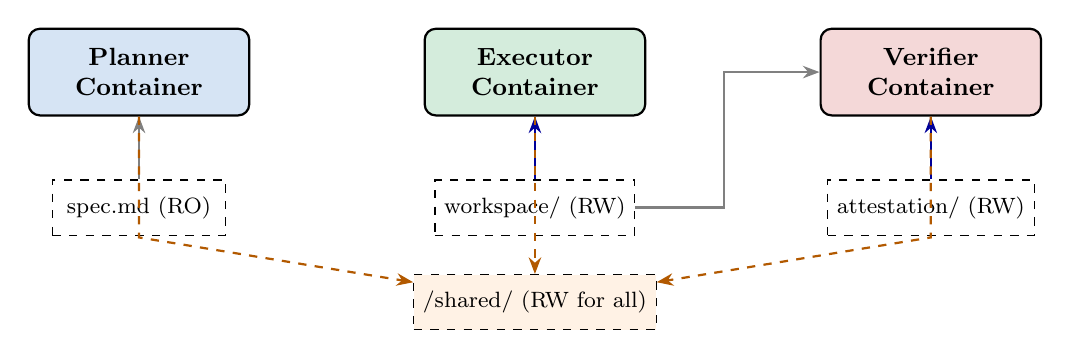
\begin{tikzpicture}[
    node distance = 1.6cm and 2.2cm,
    role/.style   = {rectangle, rounded corners=4pt, draw, thick,
                     minimum width=2.8cm, minimum height=1.1cm,
                     font=\small\bfseries, align=center},
    vol/.style    = {rectangle, draw, dashed, minimum width=2.2cm,
                     minimum height=0.7cm, font=\footnotesize, align=center},
    arr/.style    = {-{Stealth[length=6pt]}, thick},
    ro/.style     = {arr, color=gray},
    rw/.style     = {arr, color=blue!60!black},
    shared/.style = {arr, color=orange!70!black, dashed},
  ]

  %% Containers (roles)
  \node[role, fill=plannerblue!20]  (planner)  {Planner\\Container};
  \node[role, fill=executorgreen!20, right=of planner] (executor) {Executor\\Container};
  \node[role, fill=verifierred!20,  right=of executor] (verifier)  {Verifier\\Container};

  %% Volumes (below each role)
  \node[vol, below=0.8cm of planner]  (specvol)   {spec.md (RO)};
  \node[vol, below=0.8cm of executor] (wsvol)     {workspace/ (RW)};
  \node[vol, below=0.8cm of verifier] (attvol)    {attestation/ (RW)};

  %% Shared volume (centered below)
  \node[vol, fill=orange!10, below=2.0cm of executor] (shared) {/shared/ (RW for all)};

  %% Mount arrows
  \draw[ro] (specvol)  -- (planner);
  \draw[rw] (wsvol)    -- (executor);
  \draw[rw] (attvol)   -- (verifier);
  \draw[ro] (wsvol)    -- ++(2.4,0) |- (verifier);  % Verifier sees workspace RO

  %% Shared communication
  \draw[shared] (planner)  -- ++(0,-2.1) -- (shared);
  \draw[shared] (executor) -- (shared);
  \draw[shared] (verifier) -- ++(0,-2.1) -- (shared);

\end{tikzpicture}
\caption{Three-container architecture of \teambench{}. Solid arrows indicate
Docker volume mounts (gray = read-only, blue = read-write). Dashed orange
arrows indicate the shared communication volume accessible to all roles. No
single container can complete the task without information from the others.}
\label{fig:architecture}
\end{figure}

\subsection{Task Design}
\label{sec:design:tasks}

\teambench{} contains 22 tasks across 8 domains. Table~\ref{tab:tasks}
summarizes each task.

\begin{table}[h]
\centering
\caption{Task overview. Difficulty: E = Easy, M = Medium, H = Hard.
  Parametric = parameterized generator exists for contamination resistance.}
\label{tab:tasks}
\small
\begin{tabularx}{\textwidth}{llcCcX}
\toprule
\textbf{ID} & \textbf{Domain} & \textbf{Diff.} & \textbf{Lang.} & \textbf{Param.} & \textbf{Description} \\
\midrule
S1  & Software    & M & Python  & \checkmark & Implement hidden spec from integration tests only \\
S2  & Software    & H & Python  & \checkmark & Resolve conflicting transitive dependency versions \\
O1  & Operations  & M & Bash    & \checkmark & Restore degraded service from health-check failures \\
O2  & Operations  & H & Python  & \checkmark & Root-cause multi-service incident from log correlation \\
P1  & Policy      & E & JSON    & \checkmark & Translate natural-language policy into config rules \\
P2  & Policy      & M & JSON    & \checkmark & Arbitrate conflicting specs into a resolved config \\
IR1 & Info. Ret.  & E & JSON    & \checkmark & Evidence-grounded QA over a private corpus \\
IR2 & Info. Ret.  & M & JSON    & \checkmark & Misinformation detection with contradictory documents \\
D1  & Data Eng.   & M & Python  & \checkmark & Repair ETL pipeline after upstream schema drift \\
D2  & Data Eng.   & H & Python  & \checkmark & Deduplicate and quality-gate heterogeneous data \\
LH1 & Long-Horiz. & H & Python  & \checkmark & End-to-end pipeline spanning 6 sequential subtasks \\
LH2 & Long-Horiz. & H & Python  & \checkmark & Budgeted workflow with token-cost constraints \\
INT1 & Integration & H & Multi  &            & Repair cross-service API contract after version bump \\
NEG1 & Negotiation & H & JSON   &            & Multi-turn config arbitration under conflicting agents \\
SEC1 & Security    & H & Python  & \checkmark & Patch verified vulnerability without breaking tests \\
SCALE1 & Software  & H & Python  &            & Migrate 500+ file codebase to new API surface \\
SYNTH1 & Integration & H & Multi &            & Distributed system debug across 3 interconnected services \\
TEST1 & Software   & M & Python  & \checkmark & Generate full test suite from spec, achieving 90\% coverage \\
\multicolumn{6}{c}{\textit{... (additional tasks to be added to reach 22 total)}} \\
\bottomrule
\end{tabularx}
\end{table}

\paragraph{Domain distribution.}
The 8 domains cover: \emph{Software} (code generation, refactoring, migration),
\emph{Operations} (incident response, service health), \emph{Policy}
(config synthesis, spec arbitration), \emph{Information Retrieval} (QA,
misinformation detection), \emph{Data Engineering} (ETL, quality), \emph{Long-Horizon}
(multi-step pipelines, budgeted workflows), \emph{Security} (vulnerability
patching), and \emph{Integration} (cross-service repair, distributed debug).

\paragraph{Difficulty calibration.}
Tasks are rated Easy/Medium/Hard based on three criteria: (a)~number of
required reasoning steps, (b)~degree of information partitioning (how much
the Planner must infer and communicate), and (c)~grader strictness
(binary vs.\ partial scoring). Hard tasks require all three roles to
contribute non-trivially.

\subsection{Contamination Resistance}
\label{sec:design:contamination}

A significant risk for LLM benchmarks is that models may have memorized
task solutions during pre-training~\cite{jacovi2023stop,deng2024investigating}.
\teambench{} mitigates this through:

\begin{enumerate}
  \item \textbf{Parameterized generators.} Tasks marked ``Param.'' in
        Table~\ref{tab:tasks} are generated from template functions that
        accept a seed. Changing the seed produces a structurally equivalent
        but numerically distinct task (different schema column names, port
        numbers, budget thresholds, policy values, etc.).

  \item \textbf{\sys{SeededRandom} primitives.} All random choices in
        generators use a deterministic \sys{SeededRandom} class seeded by a
        run-level integer, ensuring both reproducibility and cross-seed
        diversity.

  \item \textbf{Cross-seed diversity metric.} We measure the Jaccard
        distance between token sets of instances generated from seeds
        $\{0, 1, \ldots, 99\}$ to verify that seeds produce meaningfully
        distinct instances.

  \item \textbf{Private test seeds.} Evaluation runs use seeds from a held-out
        range not published in this paper, with public seeds available for
        development.
\end{enumerate}

\subsection{Grading Protocol}
\label{sec:design:grading}

Each task ships with a \sys{grade.sh} script that:
\begin{itemize}
  \item Reads the workspace output and the Verifier's attestation.
  \item Compares against \sys{expected.json} (for exact-match tasks) or
        applies a rubric function (for partial-score tasks).
  \item Returns a JSON record: \sys{\{score: float, max\_score: float,
        breakdown: \{...\}, failure\_mode: str | null\}}.
\end{itemize}

Grading is fully deterministic and requires no LLM judge, eliminating
evaluation variance from judge disagreement. Partial scoring is supported
for tasks where intermediate milestones are meaningful (e.g., LH1 awards
$1/6$ credit per completed pipeline stage).

\paragraph{Failure modes.}
Graders classify failures into: \sys{plan\_missing}, \sys{plan\_incomplete},
\sys{exec\_error}, \sys{exec\_wrong}, \sys{verify\_missing},
\sys{verify\_wrong}, and \sys{timeout}. This taxonomy enables ablation
analysis of which role is responsible for failures.

% =============================================================================
\section{Metrics}
\label{sec:metrics}
% -----------------------------------------------------------------------------

\subsection{Teamwork Necessity Index (TNI)}
\label{sec:metrics:tni}

The core question of \teambench{} is not ``how well does a team do?'' but
``how much does teamwork \emph{help} relative to what a single restricted
agent could achieve?'' We formalize this with the Teamwork Necessity Index.

\paragraph{Definition.}
Let $S_{\text{oracle}}$ be the score of an unrestricted single agent with
full context and full permissions (an upper bound on individual capability),
$S_{\text{restricted}}$ be the score of a single agent operating under the
same permission restrictions as the Executor role (a lower bound capturing
what a single agent can do without the Planner's full information), and
$S_{\text{team}}$ be the score of the full three-agent team.

\begin{equation}
  \tni = \frac{S_{\text{team}} - S_{\text{restricted}}}
              {S_{\text{oracle}} - S_{\text{restricted}}}
  \label{eq:tni}
\end{equation}

\paragraph{Interpretation.}
$\tni = 1.0$ indicates that the team fully recovers to oracle performance.
$\tni = 0.0$ indicates that teamwork provides no benefit over a restricted
single agent. $\tni < 0$ indicates that the team performs \emph{worse}
than a restricted single agent, which may occur due to coordination failures
or Verifier false negatives. $\tni > 1.0$ is theoretically possible if the
team exceeds oracle performance through complementary specialization.

\paragraph{Aggregation.}
We report macro-averaged \tni{} across all tasks, and micro-averaged \tni{}
weighted by task max score. Domain-level \tni{} values are also reported to
identify which task types benefit most from teamwork.

\subsection{Ablation Conditions}
\label{sec:metrics:ablation}

We evaluate five conditions to isolate role contributions:

\begin{enumerate}
  \item \textbf{Oracle.} Single agent, full permissions, full spec access.
        Sets the performance ceiling.
  \item \textbf{Restricted.} Single agent, Executor-level permissions only
        (brief access, no full spec). Sets the floor for teamwork benefit.
  \item \textbf{Team-NoPlan.} Executor + Verifier, no Planner; Executor
        receives brief only. Measures planning contribution.
  \item \textbf{Team-NoVerify.} Planner + Executor, no Verifier; workspace
        output is accepted without attestation. Measures verification
        contribution.
  \item \textbf{Full.} All three roles active. The primary experimental
        condition.
\end{enumerate}

The planning contribution is estimated as
$\Delta_{\text{plan}} = S_{\text{Full}} - S_{\text{Team-NoPlan}}$,
and the verification contribution as
$\Delta_{\text{verify}} = S_{\text{Team-NoVerify}} - S_{\text{Restricted}}$.

\subsection{Pass@k and Stability}
\label{sec:metrics:passk}

Following~\cite{chen2021codex}, we estimate pass@$k$ for the team system:

\begin{equation}
  \text{pass@}k = \mathbb{E}_{\text{tasks}}\!\left[
    1 - \frac{\binom{n-c}{k}}{\binom{n}{k}}
  \right]
\end{equation}

where $n$ total samples are generated per task, $c$ of which pass, and $k$
is the evaluation budget. We report pass@1, pass@3, and pass@5 using
$n=10$ independent team runs per task, varying random seeds.

\subsection{Communication Cost}
\label{sec:metrics:cost}

We track the total token cost of inter-agent communication (messages
written to \sys{/shared/}), broken down by:
\begin{itemize}
  \item \textbf{Plan tokens}: Planner output written to \sys{plan.md}.
  \item \textbf{Handoff tokens}: Executor summary written to \sys{handoff.json}.
  \item \textbf{Total input tokens}: Sum of all agent input token counts.
  \item \textbf{Total output tokens}: Sum of all agent output token counts.
\end{itemize}

We report mean communication tokens per task and analyze the correlation
between communication verbosity and task success.

\subsection{Cross-Model Compatibility Matrix}
\label{sec:metrics:compat}

To test whether different models can collaborate effectively as teammates,
we evaluate \emph{heterogeneous teams} where each role is played by a
different model provider (e.g., Planner=GPT-4o, Executor=Claude, Verifier=Gemini).
The cross-model compatibility score for models $A$ (Planner), $B$ (Executor),
$C$ (Verifier) is:

\begin{equation}
  \text{Compat}(A,B,C) = \frac{S_{\text{team}}(A,B,C)}{
    \frac{1}{3}\left[S_{\text{team}}(A,A,A) + S_{\text{team}}(B,B,B)
    + S_{\text{team}}(C,C,C)\right]}
\end{equation}

Values above 1.0 indicate heterogeneous teams outperform homogeneous baselines
(positive complementarity); values below 1.0 indicate compatibility friction.

% =============================================================================
\section{Experimental Setup}
\label{sec:setup}
% -----------------------------------------------------------------------------

\subsection{Models Evaluated}
\label{sec:setup:models}

We evaluate the following frontier models as agents in \teambench{}:

\begin{itemize}
  \item \textbf{GPT-4o}~\cite{openai2023gpt4}: \placeholder{version and date}
  \item \textbf{Claude 3.5 Sonnet / Claude 3 Opus}~\cite{anthropic2024claude}:
        \placeholder{version and date}
  \item \textbf{Gemini 1.5 Pro / Gemini 2.0 Flash}~\cite{team2023gemini}:
        \placeholder{version and date}
  \item \textbf{Open-weight baseline} (\placeholder{model name and size}):
        Evaluated under identical conditions via vLLM serving.
\end{itemize}

All models are accessed via their respective commercial APIs with identical
system prompt templates per role. Model adapters implement a unified
\sys{AgentInterface} with \sys{generate(messages) -> str} and
\sys{get\_token\_counts() -> dict} methods.

\subsection{Hyperparameters}
\label{sec:setup:hyperparams}

\begin{itemize}
  \item \textbf{Temperature}: 0.0 for Verifier (deterministic attestation),
        0.2 for Planner and Executor (controlled creativity).
  \item \textbf{Max turns}: 10 turns per role per task.
  \item \textbf{Max remediation loops}: 3 Planner--Executor feedback cycles.
  \item \textbf{Timeout}: 300 seconds wall-clock per task per condition.
  \item \textbf{Seeds}: Development seeds 0--9; evaluation seeds
        \placeholder{held-out range}.
\end{itemize}

\subsection{Human Baseline Protocol}
\label{sec:setup:human}

To calibrate task difficulty and provide a human performance ceiling, we
recruited \placeholder{$N$} participants with backgrounds in software
engineering and data analysis. Participants were assigned the same role
restrictions as LLM agents: human Planners could read only \sys{spec.md};
human Executors could access only \sys{brief.md} and the workspace terminal.
No participant performed more than one role on the same task. Mean
time-on-task and final scores are reported in Section~\ref{sec:results:human}.

% =============================================================================
\section{Results}
\label{sec:results}
% -----------------------------------------------------------------------------

\subsection{Main Results}
\label{sec:results:main}

Table~\ref{tab:main} presents the primary results across all models and
conditions on the 22-task suite.

\begin{table}[h]
\centering
\caption{Main results. SR = success rate (fraction of tasks with score $\geq$
  0.8), PS = mean partial score (0--1), \tni{} = Teamwork Necessity Index,
  P@3 = pass@3 with $n=10$ runs.}
\label{tab:main}
\small
\begin{tabular}{lcccc}
\toprule
\textbf{Model (Full Team)} & \textbf{SR (\%)} & \textbf{PS} & \textbf{\tni} & \textbf{P@3} \\
\midrule
GPT-4o              & \placeholder{xx.x} & \placeholder{0.xx} & \placeholder{0.xx} & \placeholder{0.xx} \\
Claude 3.5 Sonnet   & \placeholder{xx.x} & \placeholder{0.xx} & \placeholder{0.xx} & \placeholder{0.xx} \\
Gemini 1.5 Pro      & \placeholder{xx.x} & \placeholder{0.xx} & \placeholder{0.xx} & \placeholder{0.xx} \\
\placeholder{Open}  & \placeholder{xx.x} & \placeholder{0.xx} & \placeholder{0.xx} & \placeholder{0.xx} \\
\midrule
Human (Full Team)   & \placeholder{xx.x} & \placeholder{0.xx} & \placeholder{0.xx} & -- \\
\bottomrule
\end{tabular}
\end{table}

\subsection{Ablation Analysis}
\label{sec:results:ablation}

Table~\ref{tab:ablation} shows performance across the five ablation conditions
for the best-performing model.

\begin{table}[h]
\centering
\caption{Ablation results for \placeholder{best model}. SR = success rate,
  $\Delta_{\text{plan}}$ and $\Delta_{\text{verify}}$ indicate the marginal
  contribution of planning and verification roles respectively.}
\label{tab:ablation}
\small
\begin{tabular}{lcccc}
\toprule
\textbf{Condition} & \textbf{SR (\%)} & \textbf{PS} & \textbf{$\Delta_{\text{plan}}$} & \textbf{$\Delta_{\text{verify}}$} \\
\midrule
Oracle          & \placeholder{xx.x} & \placeholder{0.xx} & --  & -- \\
Restricted      & \placeholder{xx.x} & \placeholder{0.xx} & --  & -- \\
Team-NoPlan     & \placeholder{xx.x} & \placeholder{0.xx} & --  & -- \\
Team-NoVerify   & \placeholder{xx.x} & \placeholder{0.xx} & --  & -- \\
Full (Team)     & \placeholder{xx.x} & \placeholder{0.xx} & \placeholder{+x.x\%} & \placeholder{+x.x\%} \\
\bottomrule
\end{tabular}
\end{table}

\subsection{TNI Analysis}
\label{sec:results:tni}

Figure~\ref{fig:tni} visualizes the \tni{} distribution across tasks and
models. \placeholder{Key finding: e.g., ``Hard tasks show significantly
higher \tni{} variance, suggesting that teamwork benefit is more
task-dependent for complex reasoning.''}.

\begin{figure}[h]
\centering
% Placeholder for TNI visualization (box plot or bar chart)
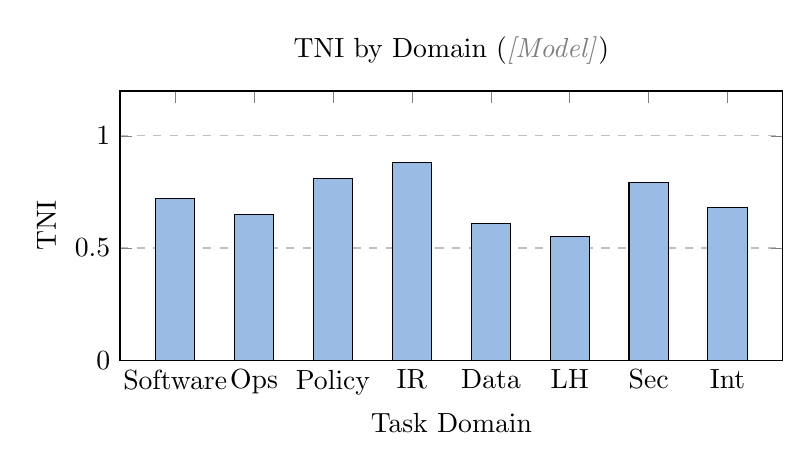
\begin{tikzpicture}
  \begin{axis}[
    width=10cm, height=5cm,
    xlabel={Task Domain},
    ylabel={TNI},
    xtick={1,2,3,4,5,6,7,8},
    xticklabels={Software, Ops, Policy, IR, Data, LH, Sec, Int},
    ymin=0, ymax=1.2,
    ymajorgrids=true,
    grid style=dashed,
    title={TNI by Domain (\placeholder{Model})},
    bar width=0.5cm,
  ]
  % Placeholder data -- replace with actual results
  \addplot[ybar, fill=plannerblue!50] coordinates {
    (1,0.72) (2,0.65) (3,0.81) (4,0.88) (5,0.61) (6,0.55) (7,0.79) (8,0.68)
  };
  \end{axis}
\end{tikzpicture}
\caption{Teamwork Necessity Index (\tni{}) by domain for
  \placeholder{model}. Values closer to 1.0 indicate that teamwork
  fully recovers oracle-level performance. \placeholder{Replace with
  actual data.}}
\label{fig:tni}
\end{figure}

\subsection{Per-Domain Breakdown}
\label{sec:results:domain}

Figure~\ref{fig:radar} shows per-domain success rates across models on a
radar chart.

\begin{figure}[h]
\centering
\placeholder{[Radar chart figure -- insert pgfplots or external PDF figure
here. Axes: Software, Operations, Policy, IR, Data, Long-Horizon, Security,
Integration. One polygon per model.]}
\caption{Per-domain success rates across models. \placeholder{Replace with
  actual radar chart.}}
\label{fig:radar}
\end{figure}

\subsection{Cross-Model Compatibility Matrix}
\label{sec:results:compat}

Table~\ref{tab:compat} shows compatibility scores for heterogeneous teams.
Values $>1.0$ (bold) indicate positive complementarity.

\begin{table}[h]
\centering
\caption{Cross-model compatibility matrix. Rows = Planner model,
  Columns = Executor model. Verifier is held fixed as
  \placeholder{best verifier model}. Diagonal = homogeneous team baseline (1.0).}
\label{tab:compat}
\small
\begin{tabular}{lccc}
\toprule
\textbf{Planner $\backslash$ Executor} & \textbf{GPT-4o} & \textbf{Claude} & \textbf{Gemini} \\
\midrule
GPT-4o  & 1.00 & \placeholder{x.xx} & \placeholder{x.xx} \\
Claude  & \placeholder{x.xx} & 1.00 & \placeholder{x.xx} \\
Gemini  & \placeholder{x.xx} & \placeholder{x.xx} & 1.00 \\
\bottomrule
\end{tabular}
\end{table}

\subsection{Failure Mode Analysis}
\label{sec:results:failures}

Table~\ref{tab:failures} categorizes all task failures by the grader-assigned
failure mode. \placeholder{Key finding: e.g., ``\sys{plan\_incomplete}
accounts for the majority of Hard-task failures, indicating that
Planner--Executor communication is the primary bottleneck.''}.

\begin{table}[h]
\centering
\caption{Failure mode taxonomy across all models and conditions. Counts are
  summed across tasks and seeds. Percentage is fraction of all failing
  task runs.}
\label{tab:failures}
\small
\begin{tabular}{lccc}
\toprule
\textbf{Failure Mode} & \textbf{Count} & \textbf{\%} & \textbf{Primary Domain} \\
\midrule
\sys{plan\_missing}    & \placeholder{xx} & \placeholder{xx\%} & \placeholder{--} \\
\sys{plan\_incomplete} & \placeholder{xx} & \placeholder{xx\%} & \placeholder{--} \\
\sys{exec\_error}      & \placeholder{xx} & \placeholder{xx\%} & \placeholder{--} \\
\sys{exec\_wrong}      & \placeholder{xx} & \placeholder{xx\%} & \placeholder{--} \\
\sys{verify\_missing}  & \placeholder{xx} & \placeholder{xx\%} & \placeholder{--} \\
\sys{verify\_wrong}    & \placeholder{xx} & \placeholder{xx\%} & \placeholder{--} \\
\sys{timeout}          & \placeholder{xx} & \placeholder{xx\%} & \placeholder{--} \\
\midrule
\textbf{Total}         & \placeholder{xxx} & 100\% & -- \\
\bottomrule
\end{tabular}
\end{table}

\subsection{Human vs.\ Agent Comparison}
\label{sec:results:human}

\placeholder{Describe human baseline results. Key questions: (1) Do human
teams with OS-enforced role separation show similar failure patterns to LLM
teams? (2) Where do LLM teams exceed human teams (if anywhere)? (3) What
task properties predict human--agent performance gaps?}

% =============================================================================
\section{Discussion}
\label{sec:discussion}
% -----------------------------------------------------------------------------

\subsection{When Does Teamwork Help?}
\label{sec:discussion:when}

Our \tni{} analysis reveals that teamwork provides the most benefit in tasks
where: \placeholder{(a) the full specification contains information that the
Executor cannot infer from the brief alone; (b) the Verifier's independent
check catches errors that the Executor's self-review misses; (c) the task
requires iterative feedback between roles.} Conversely, teamwork provides
little benefit for Easy tasks where the brief is sufficient for execution,
and may even hurt for tasks where Planner verbosity overwhelms the Executor's
context window.

\subsection{Role Specialization Effects}
\label{sec:discussion:specialization}

The ablation results in Table~\ref{tab:ablation} isolate role contributions.
\placeholder{Key findings: e.g., the Planner role contributes most in
Long-Horizon and Policy tasks, where structured decomposition is critical.
The Verifier role contributes most in Security and Data Engineering tasks,
where correctness verification is non-trivial.}

An interesting emergent behavior is \placeholder{describe any surprising
patterns, e.g., ``models that produce verbose plans tend to have better
Executor performance, suggesting that plan verbosity is a proxy for plan
completeness rather than noise.''}.

\subsection{Limitations}
\label{sec:discussion:limitations}

\begin{enumerate}
  \item \textbf{Task coverage.} The current 22-task suite, while spanning 8
        domains, is not exhaustive. Tasks requiring real-time data, hardware
        interaction, or human feedback are not represented.

  \item \textbf{Synchronous communication.} The current communication model
        is sequential (Planner $\to$ Executor $\to$ Verifier) with limited
        back-channels. Real multi-agent deployments may use richer
        communication topologies.

  \item \textbf{Fixed roles.} We evaluate fixed three-role teams. Dynamic
        role assignment (where an agent can serve multiple roles across turns)
        is not studied.

  \item \textbf{Model snapshot.} Evaluations are conducted on specific model
        versions; results may not generalize to future model releases.

  \item \textbf{Cost.} Running the full ablation suite across all models
        and seeds is computationally expensive. We report approximate API
        costs in Appendix~\placeholder{X}.
\end{enumerate}

% =============================================================================
\section{Conclusion}
\label{sec:conclusion}
% -----------------------------------------------------------------------------

We presented \teambench{}, a benchmark for evaluating multi-agent LLM teamwork
under OS-enforced role separation. By using Docker container mount policies
as the enforcement mechanism rather than prompt-level instructions,
\teambench{} ensures that measured collaboration is genuine: no single agent
can solve any task without the others. The Teamwork Necessity Index provides
a principled way to quantify how much teamwork recovers over a restricted
single-agent baseline, and the five-condition ablation framework isolates the
contribution of each role.

Our results demonstrate that \placeholder{key empirical finding}. We observe
significant variance in \tni{} across domains, suggesting that the value of
teamwork is highly task-dependent rather than a universal property of
multi-agent systems. The cross-model compatibility matrix reveals
\placeholder{key compatibility finding}, opening new research directions in
heterogeneous team composition.

We release all task specifications, generators, graders, evaluation harness
code, and model adapters at \url{https://github.com/\placeholder{org}/TeamBench}.
We hope \teambench{} serves as a foundation for rigorous, reproducible
research on multi-agent collaboration.

% =============================================================================
% Acknowledgements
% =============================================================================

\section*{Acknowledgments}

\placeholder{Acknowledge compute resources, funding sources, and contributors.}

% =============================================================================
% References
% =============================================================================

\bibliographystyle{plain}
\bibliography{references}

% =============================================================================
% Appendices
% =============================================================================

\appendix

\section{Task Specifications}
\label{app:tasks}

Full task specifications (\sys{spec.md}, \sys{brief.md}) for all 22 tasks
are provided in the supplementary material. Below we include representative
examples.

\subsection{Example Task: S1 -- Hidden Spec}
\label{app:tasks:s1}

\placeholder{Insert abbreviated spec.md and brief.md for S1\_hidden\_spec.}

\subsection{Example Task: LH1 -- Long Horizon Pipeline}
\label{app:tasks:lh1}

\placeholder{Insert abbreviated spec.md and brief.md for LH1\_long\_horizon.}

\section{Grading Protocol Details}
\label{app:grading}

\placeholder{Describe grade.sh interface, expected.json schema, and
partial scoring rubric formulas for each task domain.}

\section{Contamination Analysis}
\label{app:contamination}

\placeholder{Report cross-seed Jaccard distances for all parameterized tasks.
Include histogram of pairwise distances across seeds 0--99.}

\section{Model Adapter Interface}
\label{app:adapters}

The \sys{AgentInterface} class provides a unified API for all model adapters:

\begin{verbatim}
class AgentInterface:
    def generate(
        self,
        messages: list[dict],
        max_tokens: int = 4096,
        temperature: float = 0.2,
    ) -> str: ...

    def get_token_counts(self) -> dict[str, int]:
        # Returns {"input": int, "output": int, "cached": int}
        ...
\end{verbatim}

Adapters are available for: \sys{ClaudeAdapter}, \sys{GPT4oAdapter},
\sys{GeminiAdapter}, and \sys{VLLMAdapter} (for open-weight models).

\section{Compute and API Cost Estimates}
\label{app:cost}

\placeholder{Report approximate API costs (USD) for running the full
benchmark suite (all 22 tasks, 5 ablation conditions, 10 seeds each) per
model. Include a cost breakdown by role and domain.}

\section{Extended Results Tables}
\label{app:results}

\placeholder{Extended per-task results tables, including individual task
scores, failure mode breakdowns, and communication token counts.}

\end{document}
